\chapter{Results}

\begin{figure}[htbp]
    \centering
    \begin{subfigure}{.5\textwidth}
        \centering
        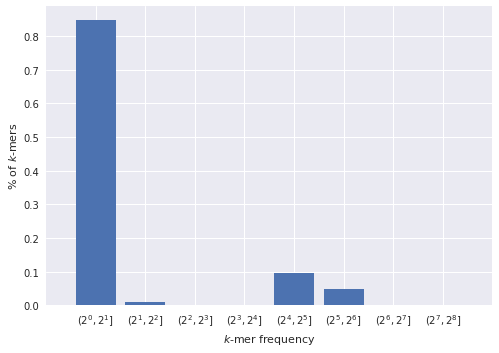
\includegraphics[width=\textwidth]{figures/e_coli-kmer_frequencies-exact-K31}
        \caption{Exact frequencies}
    \end{subfigure}%
    \begin{subfigure}{.5\textwidth}
        \centering
        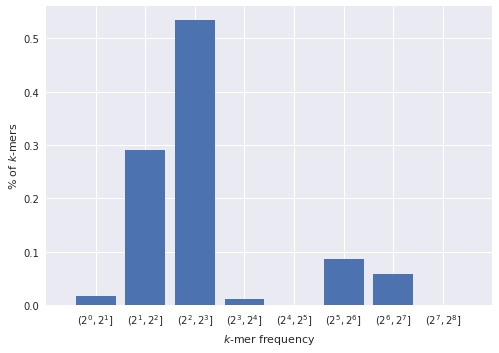
\includegraphics[width=\textwidth]{figures/e_coli-kmer_frequencies-estimated-K31-W20000000}
        \caption{Estimated frequencies}
    \end{subfigure}
    \begin{subfigure}{.5\textwidth}
        \centering
        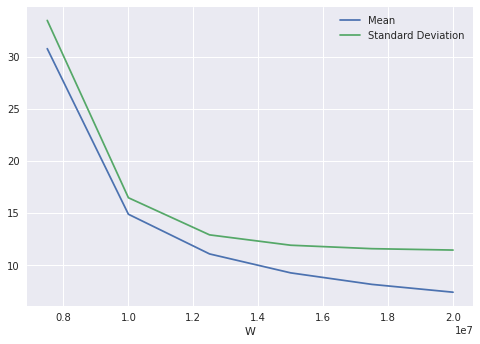
\includegraphics[width=\textwidth]{figures/e_coli-error_mean_stddev-K31-D8-T40}
        \caption{Error mean and standard deviation as a function of $W$}
    \end{subfigure}
	\caption{\kmer frequencies for \emph{E.~Coli} genome with $k=31$. \dBCM parameters: $(W=20M, D=8)$}\label{fig:ecoli-exact-frequencies}
\end{figure}

\begin{figure}[htbp]
	\centering
    \begin{subfigure}{.5\textwidth}
        \centering
        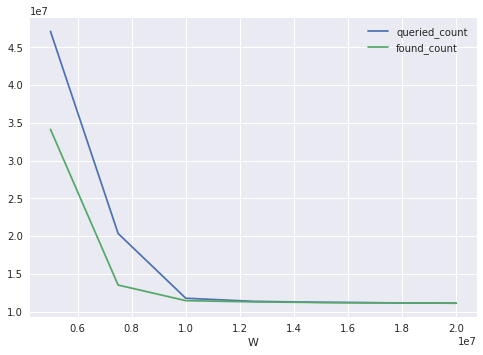
\includegraphics[width=\textwidth]{figures/e_coli-queried_and_found-K31-D8-T40}
        \caption{Queried \& Found}\label{subfig:ecoli-queriedandfound}
    \end{subfigure}%
    \begin{subfigure}{.5\textwidth}
        \centering
        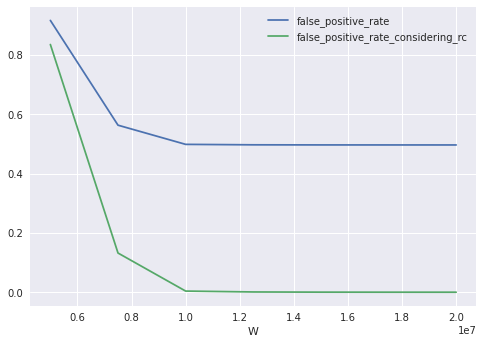
\includegraphics[width=\textwidth]{figures/e_coli-false_positive_rates-K31-D8-T40}
        \asq{Vale manter os dois, ou melhor só colocar o erro considerando RC como true positive para reduzir clutter?}
        \caption{False Positives}\label{subfig:ecoli-falsepositives}
    \end{subfigure}
	\caption{Number of (a) \kmer{s} queried and found during traversal and (b) false positives}\label{fig:ecoli-exact-frequencies}
\end{figure}